


%%%%%%%%%%%%%%%%%%%%%%%%%%%%%%%%%%%%%%%%%%%%%%%%%%%%%%%%%%%%%%%
%
% Welcome to Overleaf --- just edit your LaTeX on the left,
% and we'll compile it for you on the right. If you open the
% 'Share' menu, you can invite other users to edit at the same
% time. See www.overleaf.com/learn for more info. Enjoy!
%
%%%%%%%%%%%%%%%%%%%%%%%%%%%%%%%%%%%%%%%%%%%%%%%%%%%%%%%%%%%%%%%
\documentclass{article}
\usepackage{CJKutf8}
\usepackage{graphicx}
\usepackage{amsmath}
\usepackage{xcolor}
\usepackage{fancyhdr}
\usepackage{hyperref}
\usepackage{tcolorbox}
\usepackage{setspace}
\pagestyle{fancy}
\fancyhf{}
\rfoot{\thepage}
\begin{document}
\begin{CJK*}{UTF8}{gbsn}
% {\centering\textbf{\fontsize{16}{20}\selectfont shallow system}\par}

\section*{Convectively coupled equatorial waves}

\subsection*{简介}


对流耦合赤道波动控制了热带一部分的降水变率,其水平结果和频散特征来自于Matsuno's(1966)在赤道$\beta$ 平面上的浅水方程的解,包括:
\begin{enumerate}
    \item 
    kelvin wave
    \item
    equatorial Rossby wave
    \item
    mixed Rossby-gravity  wave
    \item
    inertio-gravity wave
\end{enumerate}

\

由于存在湿过程的影响,他们的倾斜垂向结构是复杂的,而且他们的尺度与理论干波的期望的结构不一致。

\

CCEWs的动力结构和云形态在一个令人惊讶的大尺度范围内显示出很大程度的自相似性,其前缘为浅对流,其次是深对流,然后是层云降水,反映了单个中尺度对流复合体的特征。

\

CCEWs在热带地区具有广泛的影响,其在一般环流模式中的模拟仍然存在问题,尽管使用更简单的模式已经取得了进展。对CCEWs的完整理解仍然是热带气象学的一个挑战。

\

目前,CMIP6 的众多模式数据中,仍然无法较好的抓住赤道波动。

\

\subsection*{ 研究回顾}

\

积云降水在热带地区中的降水占绝大部分,如果没有卫星观测,你会感觉许多降水看起来是随机分布的。只有在一些特别的区域(如季风区),才会观察到一些相对低频的周期性降水(一个月左右)。

\ 

事实上,热带的对流降水被认为在广阔的时空尺度上是有组织的,从中尺度对流系统(MCSs)到行星尺度的特征(MJO)。在中尺度上,降水往往是由向东或者是向西的波动组成,无论是沿着赤道海上在热带辐合带内(ITCZ)与之平行的纬度范围内。

\ 


与热带外地区不同,赤道地区可以为扰动提供发展背景的观点最早可以追溯到Riehl[1945],他认为西传的波动导致了加勒比地区的许多日常天气变率。

\

这种“东风波”(Easterly waves,EWs)被定义为热带辐合带内向西传播的几千公里尺度的低压反向的槽,并将其与热带气旋联系起来(Dunn[1940],Riehl[1948])。
后续的研究也证实了,东风波或者称为热带低压型扰动是印度洋以外热带几乎所有地区的重要特征。

\ 

在20世纪50年代后期,人们认识到旋转行星的低纬度区域会产生一类特殊的沿赤道的"被捕获"的运动[Yoshida, 1959; Rosenthal, 1960, 1965; Bretherton, 1964].

在最经典的赤道运动的文献中,松野[1966]求解了赤道$\beta$平面下浅水方程组的纬向传播的波解,该方程在恢复力为重力和线性变化的科氏力控制的一层定常密度流体中的运动。根据这个系统的解,得到了现在熟知的赤道大气和海洋的波动,即
\begin{enumerate}
    \item 
    kelvin wave
    \item
    equatorial Rossby wave
    \item
    mixed Rossby-gravity  wave
    \item
    westward and eastward inertio-gravity wave (WIG and EIG)
\end{enumerate}

\ 


在其文章发表时,在赤道平流层对于MRG波[Yanai and Maruyama, 1966; Maruyama, 1967]和kelvin波[Wallace and Kousky, 1968]的观测证据还没有被证实。
这些热带大气模态的发现, 以及后续发展的著名的海洋模态,Gill响应[Wunsch and Gill, 1976]是赤道浅水理论的重要突破。

\

其中,MRG波主要与经向流波动有关,而Kelvin波主要表现为纬向波动。这些被观测到的平流波动也被认为是“干”模态,认为没有和水汽耦合或者其他强迫。它们的初始能量源被假定为\textbf{对流层中湿对流的非绝热加热},因为它们的垂直结构表明向上的能量频散,与下面的强迫一致[Holton, 1972, 1973]。

\ 

平流层干Kelvin波和MRG波的发现,激发了人们极大的兴趣来确定这些模态的潜力,以解释平流层准两年振荡( QBO )的工作,即平流层低层向下传播的西风向东风气流转变的显著周期变化,周期为22个月左右[\textit{Baldwin} et al . , 2001]。

\ 

后续几年,随着卫星数据被用来探测云团中西传和东传的扰动[Chang,1970;Yanai and Murakami, 1970a, 1970b; Wallace and Chang, 1972; Reed and Recker, 1971],激发了对流耦合对应浅水理论干模态的可能性。与此同时,光谱研究解释了了季节内振荡(MJO)[Madden and Julian 1971, 1972],由一个约10000 km尺度的深对流和多云的包络组成,东传相速度在$4~8 m s^{-1}$,并与大尺度环流相耦合.该包络一定程度上被认为是有组织的对流耦合赤道波动,伴随着MCSs的光谱。此外,更详细的关于卫星降水云团数据的研究Gruber [1974], Zangvil [1975], and Zangvil and Yanai [1980, 1981],进一步证实了赤道浅水模态与深对流之前的强烈联系。

\ 

尽管这些研究为对流耦合ER、MRG和Kelvin波的存在提供了充分的证据,但直到20世纪90年代才对它们进行了详细的观测研究,此时对MJO和干平流层模态的研究仍在继续。随着长周期全球卫星和业务数据的积累,Liebmann and Hendon [1990], Hendon and Liebmann [1991], and Takayabu and Nitta [1993]分离出了对流耦合MRG波的性质,并表明\textbf{它们的垂直结构在对流层中低层表现出随高度的强烈倾斜},这与Reed和Recker [ 1971 ]研究的EWs非常相似。此外,更多的证据也表明了存在不同种类的Kelvin和MRG模式,其中一些是主要在平流层中出现的相对快速传播的干燥模式,而另一些是在对流层中与对流紧密耦合的更慢速传播的波Takayabu and Murakami [1991]。

\ 

Takayabu [ 1994a ]对高分辨率地球同步卫星图像进行了时空谱分析,检测到了与Kelvin波、ER波、MRG波和WIG波相对应的谱峰。Wheeler and Kiladis [ 1999 ] (以下简称WK99)在Takayabu [ 1994a ]的工作基础上,建立了全球时空谱。图1显示了这样一种光谱,它是由卫星亮温中的原始功率除以其红色噪声背景(详见WK99)的估计得到的。

\begin{figure}
    \centering
    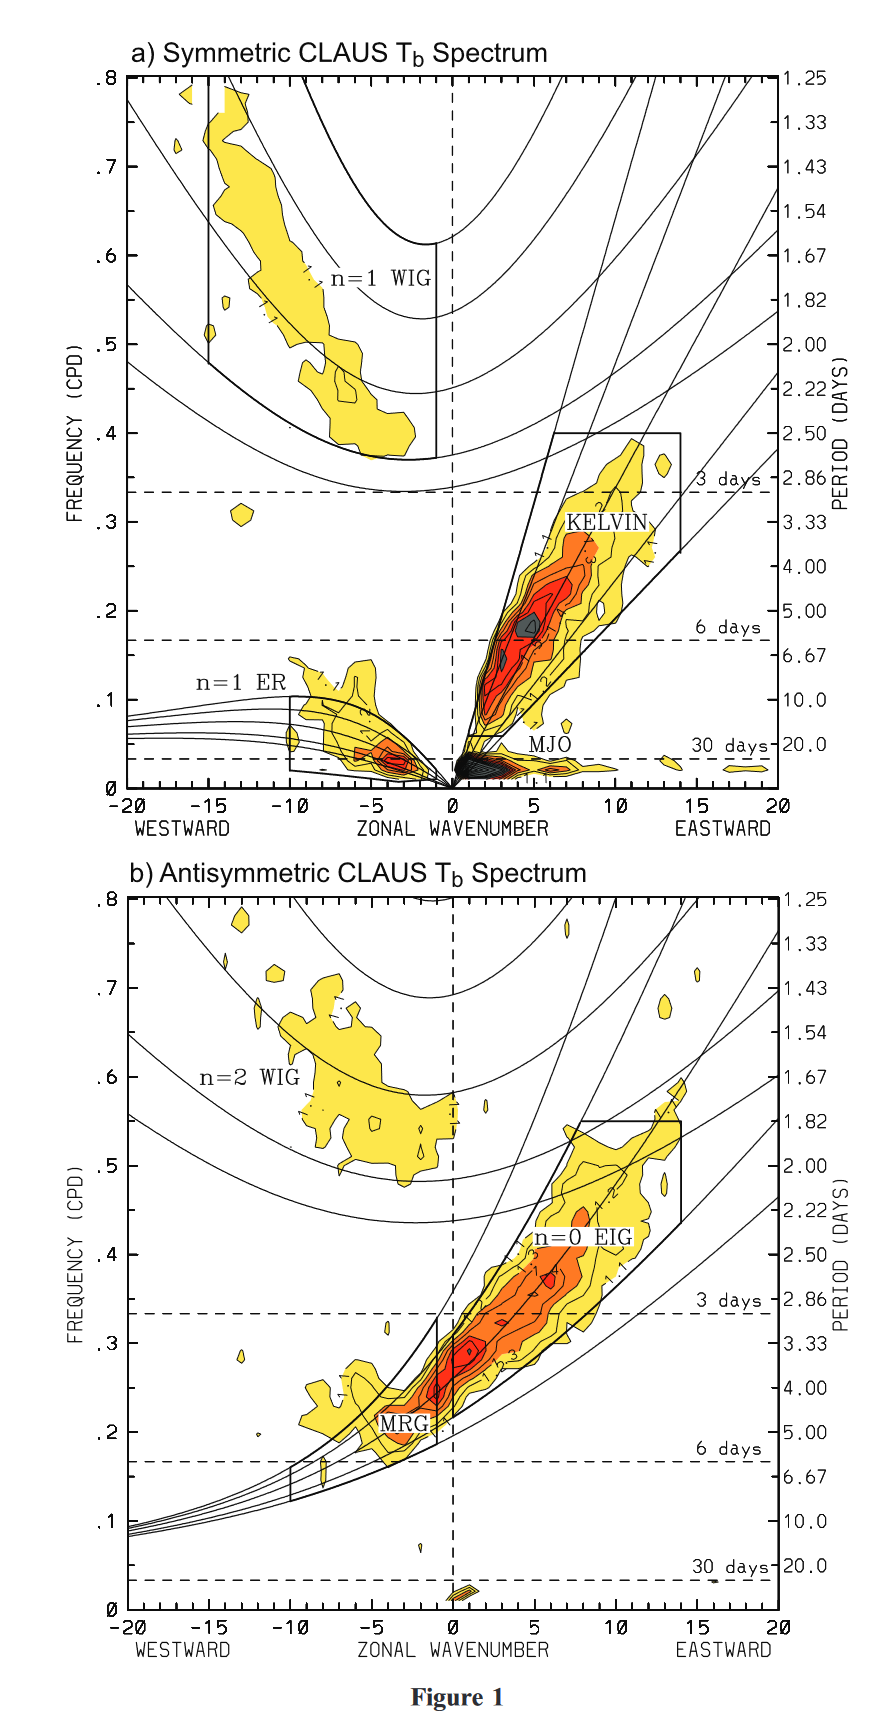
\includegraphics[width=0.75\linewidth]{Fig1.png}
    \caption{Enter Caption}
    \label{fig:enter-label}
\end{figure}

\ 

值得注意的是,这些CCEW的频散特性和结构与线性理论预测的频散特性和结构大体一致,即使不考虑基态流的潜在影响,也不考虑与对流耦合产生的非线性。


\ 


\subsection*{对流耦合赤道波动经典理论}


\ 

\subsubsection*{2.1 浅水理论}


\ 

如前文所述,一部分热带深对流似乎是受动力学控制的,这与松野[ 1966 ]的SW理论相一致。但是应用这些理论到观测到的CCEWs仍然是缺少证据的[e.g., Lindzen, 2003]。


\ 

SW方程描述了旋转球体上单层不可压缩、均匀密度流体的垂向独立运动,也称为拉普拉斯潮汐方程。SW方程可以从完整的原始方程中流的垂直与水平和时变部分的数学分离中推导出来,尽管进行这种分离和推导运动的垂直依赖性所需的假设远非微不足道。


\ 

松野[ 1966 ]考虑了关于静止基本状态线性化的无粘SW方程。科里奥利参数f被假设为与赤道(即f = $\beta$y)的距离成线性比例,赤道(即f = $\beta$y)是热带地区运动的一个适当有效的近似。公式为


\ 

\[\frac{\partial u_l}{\partial t} - \beta yv_l = - \frac{\partial \phi_l}{\partial x},\quad(1)
\]


\ 


\[ \frac{\partial\nu_l}{\partial t}+\beta yu_l=-\frac{\partial\phi_l}{\partial y},\quad(2)\]

\ 

\[ \frac{\partial\phi_l}{\partial t}+gh_e\left(\frac{\partial u_l}{\partial x}+\frac{\partial\nu_l}{\partial y}\right)=0.\quad(3) \]


\ 

其中,$u_l$ 和 $v_l$  是纬向和经向的速度,$\phi_l$是位势,g 是重力加速度,$h_e$是
流体的深度。方程( 1 )和( 2 )是水平动量方程,( 3 )是质量守恒的结果,将位势的变化与散度联系起来。我们用下标l表示在全三维大气流动的背景下,这些方程只模拟水平( x和y)和时间( t )变化的流动分量。也就是说,它们控制着一个特定的垂直模态的运动,l,为此他必须做出适当的选择。



\ 

松野[ 1966 ]首次得到了这些方程[see also Andrews et al., 1987; Gill, 1982a; Pedlosky, 1987; Wheeler, 2002; Holton, 2004].的完整的带传播波解。简而言之,寻求该形式的纬向传播波解:


\ 

\[\left.\left(\begin{array}{c}u_l\\v_l\\\phi_l\end{array}\right.\right)=\left(\begin{array}{c}\hat{u}(y)\\\hat{v}(y)\\\hat{\phi}(y)\end{array}\right)\exp[i(kx-\omega t)],\quad\quad\quad(4)\]


\ 

其中,k是纬向波数,$\omega$是频率,代入得到$\hat{v}$中的二阶微分方程:


\ 

\[\left.\frac{d^2\hat{\nu}}{dy^2}+\left(\frac{\omega^2}{gh_e}-k^2-\frac k\omega\right.\beta-\frac{\beta^2y^2}{gh_e}\right)\hat{\nu}=0.\quad\quad\quad(5)\]


\ 

这个方程远离赤道衰减的解是众所周知的,从中可以看出括号中的系数的常数部分必须满足


\ 

\[\frac{\sqrt{gh_e}}\beta\left(\frac{\omega^2}{gh_e}-k^2-\frac k\omega\beta\right)=2n+1\quad n=0,1,2,\ldots.\quad(6)\]

\ 

这个方程对于每一个整数n,都给定了一个关于k和$\omega$之间的关系,也被认为是波动的频散关系.方程关于$\omega$为3次方,得到EIG、WIG和ER波对应的3类解。对于n = 0的解需要特别考虑,对应于MRG波。此外,将( 1 ) - ( 3 )未被( 5 )覆盖的另一个解对应着kelvin波,当$\hat{v} =0$,对于所有的y,为了与(6)一致,将其标记为n=1.关于( 6 )的所有解,以及Kelvin波频散关系,在图2中给出


\ 

\begin{figure}
    \centering
    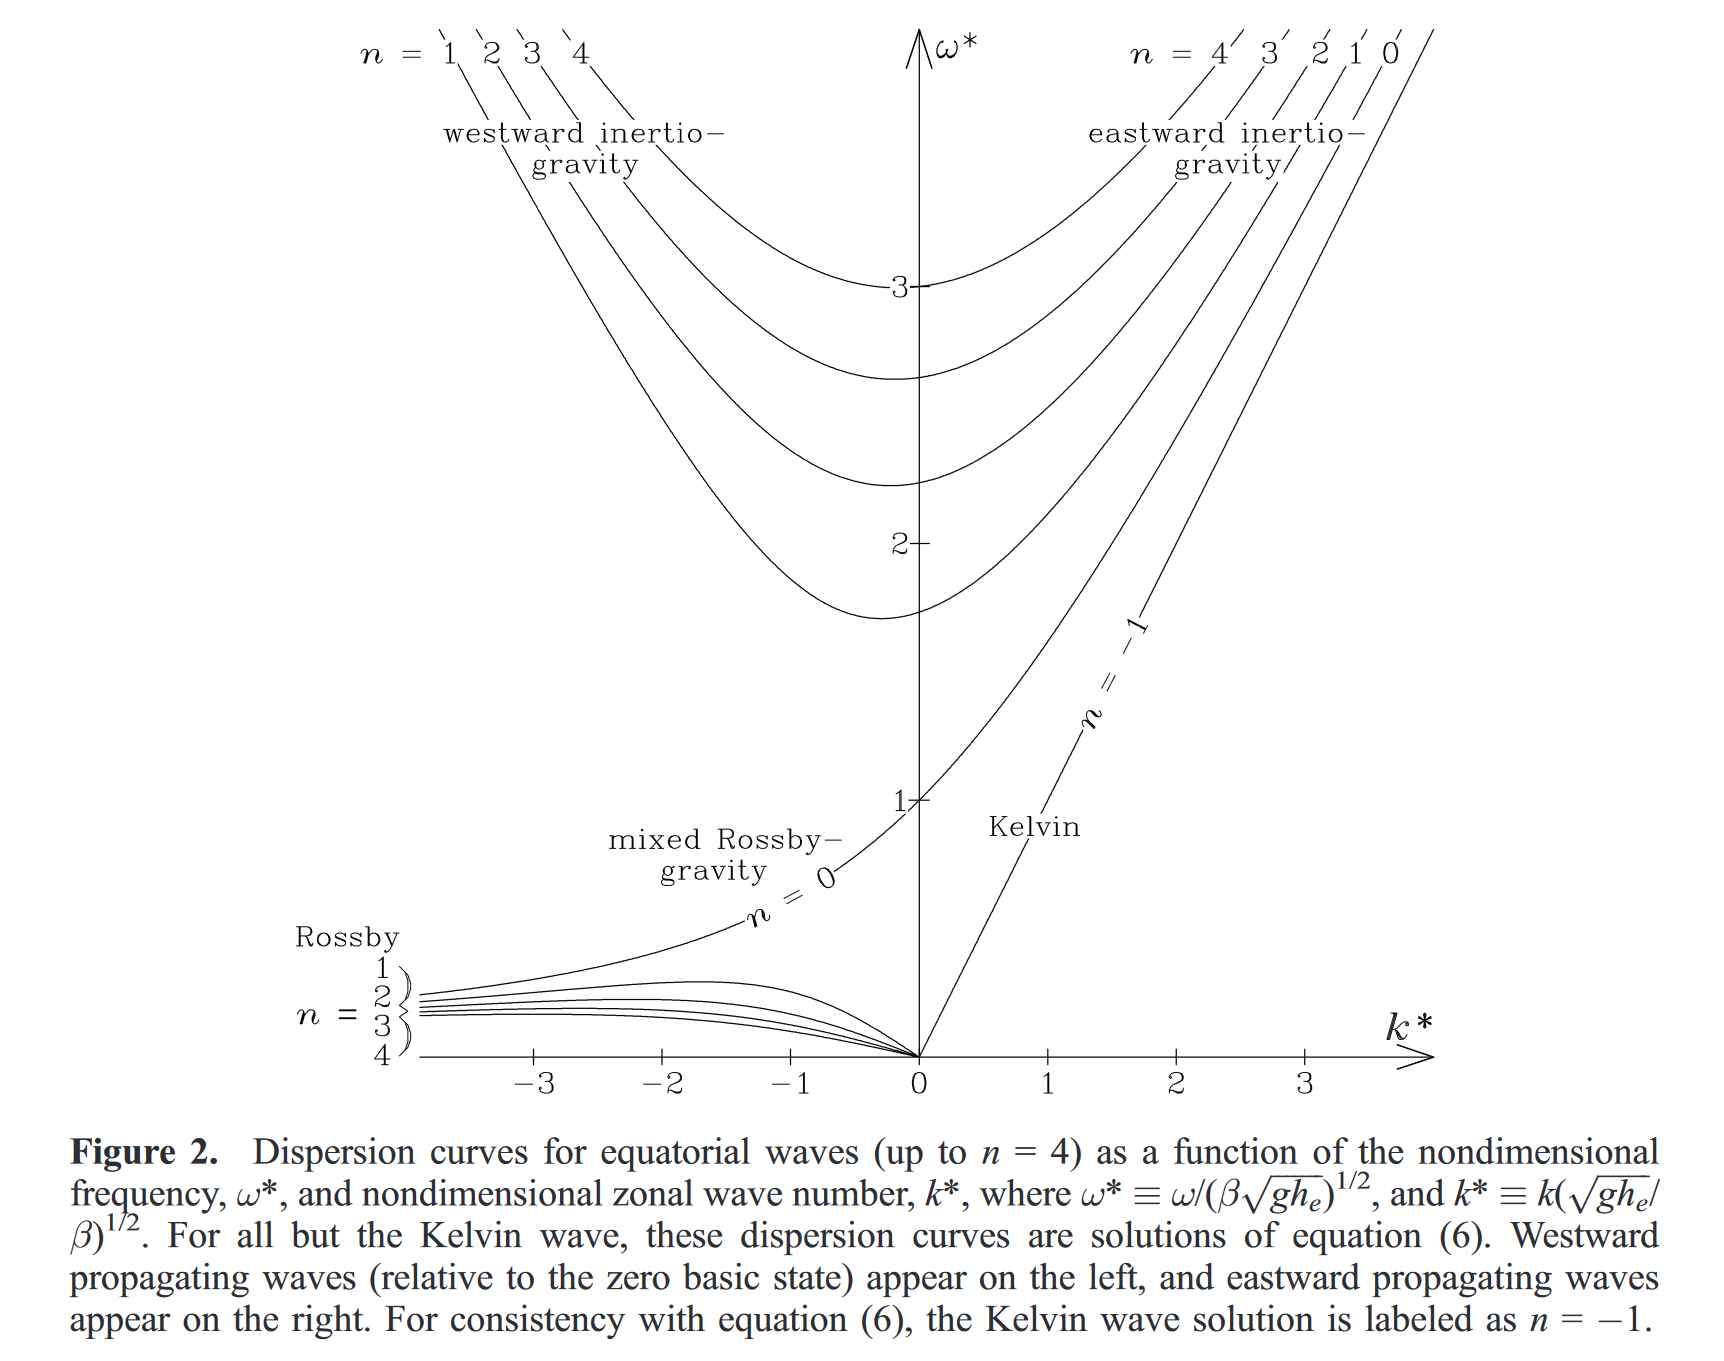
\includegraphics[width=0.75\linewidth]{Fig2.png}
    \caption{Enter Caption}
    \label{fig:enter-label}
\end{figure}


\ 

将式(5)中$\hat{v}$的解,代回式(1)~式(3),就可以得到波解的水平结构。图3展示了Kelvin波,n = 1 ER波,MRG波,n = 0 EIG波,n = 1和n = 2 WIG波的完整结构。由于n对应于v (除Kelvin波外)经向剖面的节点数,故称其为经向模态数。这六种波型包括了所有被观测到的CCEW。其他赤道波动模态的水平结构都要复杂得多[Wheeler, 2002].


\ 

\begin{figure}
    \centering
    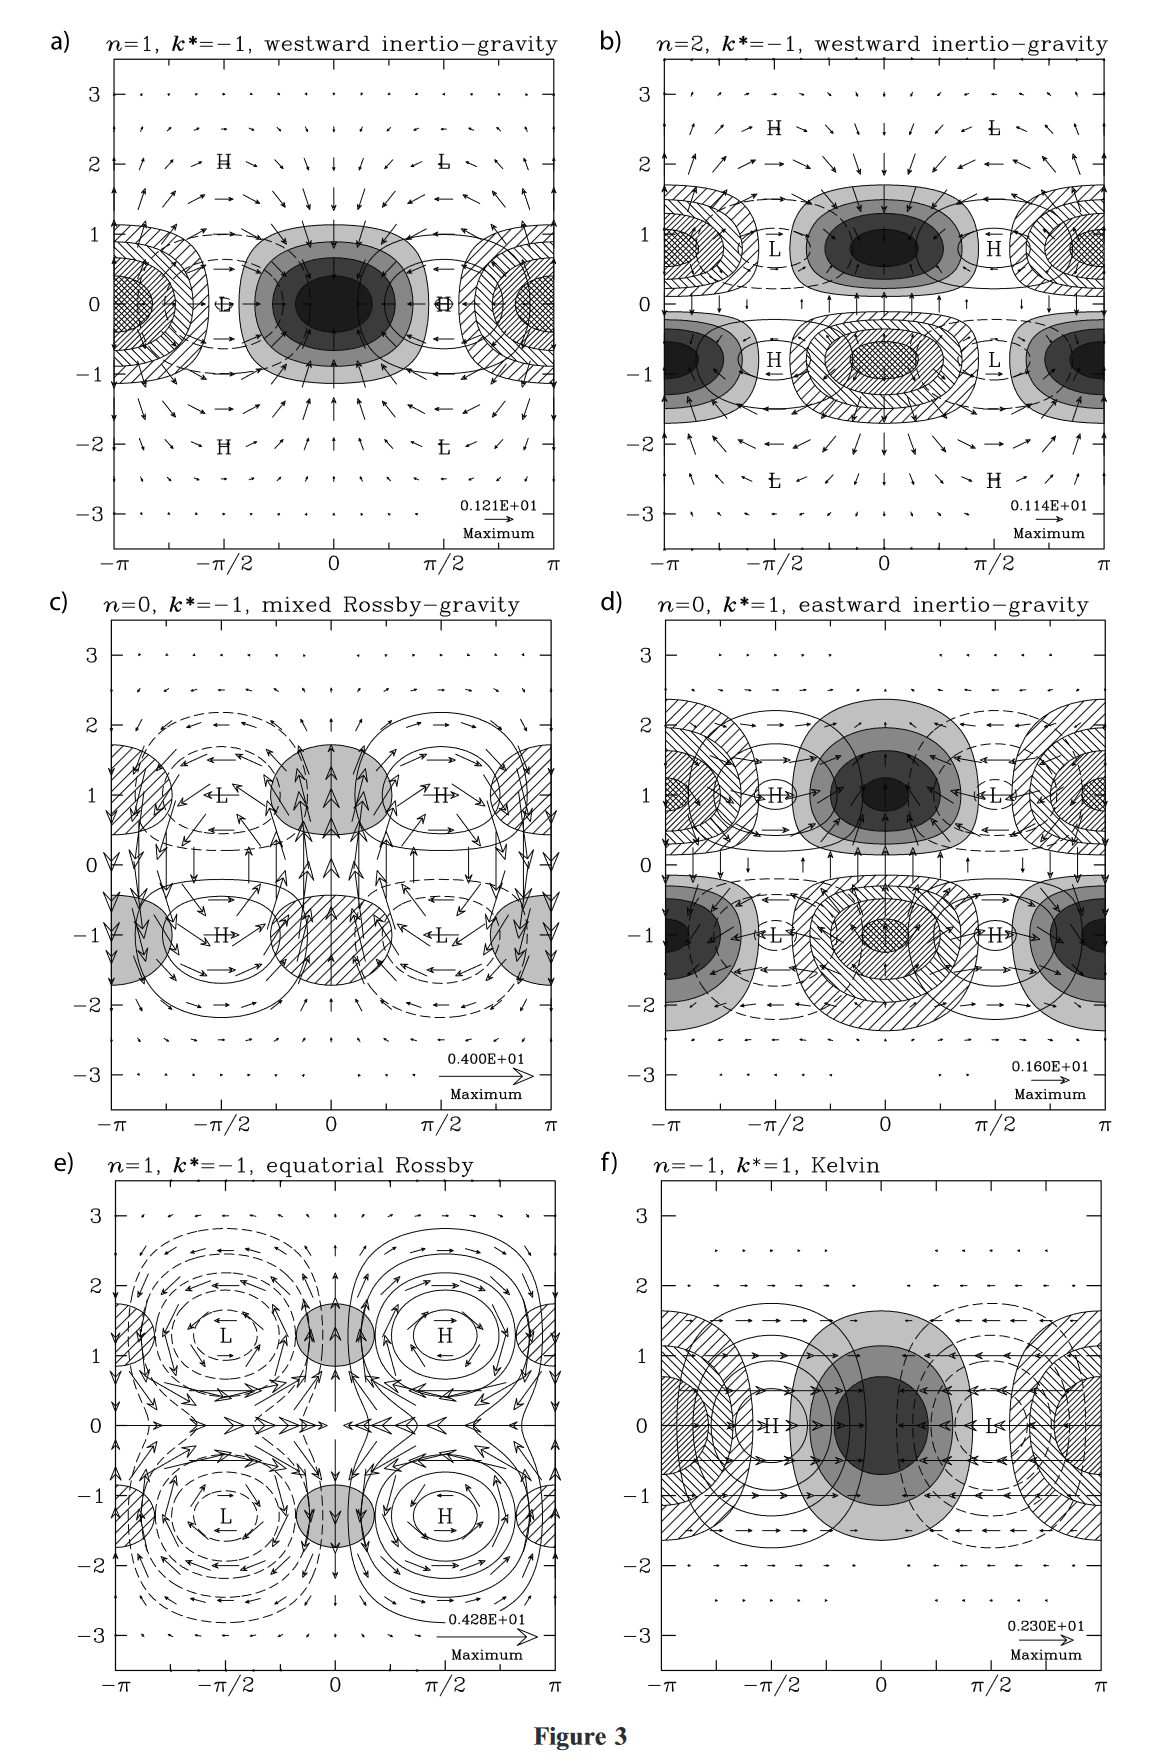
\includegraphics[width=0.75\linewidth]{Fig3.png}
    \caption{Enter Caption}
    \label{fig:enter-label}
\end{figure}


\ 


\begin{enumerate}
    \item 由于原始的SW方程是线性化的,因此波解的任何线性组合也是一个解。
    \item 非频散波Kelvin波的相速度为$c=\sqrt{gh_e}$,所有类型的惯性重力波,无论向东还是向西,当k较大时,其相速度都渐近接近这一量级。
    \item 赤道Rossby形变半径由$Re=(\sqrt{gh_e}/\beta)^{1/2}$给出,它控制着解随离赤道距离的衰减速率,并被用来衡量图3中的水平长度。在实际应用中,CCEWs (见表1)的Re在纬度10 °量级。
    \item 波的水平能量频散由群速度$c_g^{(x)}\equiv \partial \omega / \partial k$决定,这可以从图2中估计出来。例如,MRG波具有向西的相位传播( $\omega$ / k为负数),但向东的能量频散( $c_g^{(x)}$决为正)。
    \item 惯性重力波和Kelvin波的特征更趋向于发散,而MRG波和ER波的特征更趋向于旋转。
    \item 浅水深度$h_e$决定了波动的速度和尺度,对于整个大气层被称为等效深度(equivalent depth)
\end{enumerate}

\ 

\begin{figure}
    \centering
    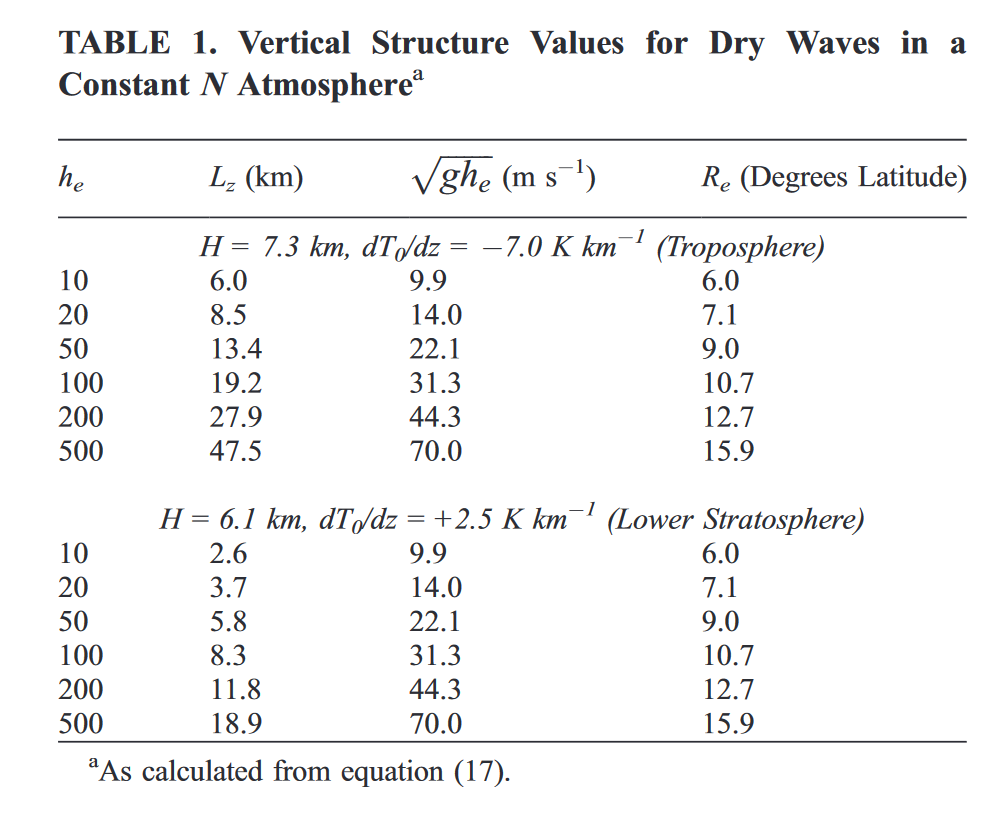
\includegraphics[width=0.75\linewidth]{table1.png}
    \caption{Enter Caption}
    \label{fig:enter-label}
\end{figure}


\ 


\subsubsection*{2.2 将浅水方程和大气运动联系起来}

\ 

虽然 SW 理论对 CCEW 的适用性是显而易见的,但既没有独特的也没有标准的方法将大气运动的完整三维方程与 SW 运动方程联系起来,特别是当环流受到对流加热的强制或耦合时。 相反,有多种方法可以导出这种关系,其不同之处在于垂直结构的选择和包含非绝热效应的方式。 在这里,我们总结了几种可能性,并注意到不同选择对相应理论色散特性和波浪结构的影响。


\ 

\paragraph*{2.2.1 干波}


\ 

当忽略水汽的影响,特别是由于冷凝和蒸发而导致的加热和冷却时,导出其水平结构由 SW 方程控制的大气波的解相对简单。 考虑具有对数压力垂直坐标 z 的流体静力学基元方程 [e.g., Holton, 2004, p. 317],,关于静止基本状态的线性化:


\ 

\[\begin{aligned}
\begin{aligned}\frac{\partial u}{\partial t}-f\nu+\frac{\partial\phi}{\partial x}\end{aligned} =0, & \left(7\right)  \\
\frac{\partial\nu}{\partial t}+\textit{fi}+\frac{\partial\phi}{\partial y} =0, & \left(8\right)  \\
\frac{\partial u}{\partial x}+\frac{\partial\nu}{\partial y}+\rho_0^{-1}\frac{\partial(\rho_0w)}{\partial z}=0,& \left(9\right) 
\end{aligned}\]


\ 

\[\frac\partial{\partial t}\left(\frac{\partial\phi}{\partial z}\right)+wN^2=0,\quad\quad\quad\quad\quad(10)\]


\ 

其中 $z=-Hlog(p/p_s)$,p 为压力,下标 s 表示固定表面值,$w$ 为垂直速度,$H = RT_m/g $为一层平均温度 $T_m$ 的刻度高度,R 为气体常数 , $\rho_0(z)  = \rho_s exp(-z /H) , N^2 = (R/H)(dT_0 /dz+g/c_p)$ 是静态稳定性的度量,其中 $dT_0/dz$ 是平均失效率,$c_p$ 是 恒压下干燥空气的比热。 为简单起见,我们假设 $N^2$ 是恒定的,并且忽略加热和摩擦效应。 结合(9)和(10)消除w,


\ 

\[\frac\partial{\partial t}L[\phi]-N^2\left(\frac{\partial u}{\partial x}+\frac{\partial\nu}{\partial y}\right)=0,\quad\quad\quad\quad(11)\]


\ 

其中 $L=(1/\rho)(\partial /\partial z)(\rho_0)(\partial / \partial z)$ 是线性运算符。 现在假设 $\phi$ 具有垂直结构$\phi_v$,即 L 的本征函数; 那是,


\ 


\[L[\phi_{\nu}]=-\lambda\phi_{\nu},\quad\quad\quad\quad\quad\quad\quad(12)\]

\ 


其中,$\lambda$是常数,式(11)变为:


\ 


\[\frac{\partial\phi}{\partial t}+\frac{N^2}\lambda\left(\frac{\partial u}{\partial x}+\frac{\partial\nu}{\partial y}\right)=0.\quad\quad\quad\quad\quad(13)\]


\ 

请注意,(7)、(8) 和 (13) 在代数上等价于 SW 方程 (1) – (3),其等效深度为:



\ 

\[h_e=N^2/(g\lambda)\quad\quad\quad\quad\quad\quad\quad(14)\]


\ 

并且该等价性与通过 f 平面或 $\beta$ 平面近似科里奥利参数的方法无关。 因此,我们可以构造 (7) – (10) 的解,其水平结构来自 SW 方程的解,其垂直结构来自 L 的本征函数。我们可能期望这些解能够提供有关结构和色散性质的见解 观察到的 CCEW。 然而,第一个复杂之处是,即使对于干波,也有两种根本不同类型的垂直结构,它们是 L 的本征函数:


\ 


\[\exp(z/2H)\exp(imz)\quad\quad\quad\quad(15\text{a})\]


or


\ 

\[\exp(z/2H)\sin(mz+b)\quad\quad\quad\quad(15\text{a})\]



\ 

其中 m 是垂直波数,b 是相位(常数)。 第一个结构 (15a) 用于辐射上边界条件 [Lindzen, 1974, 2003],而 (15b) 用于上边界处的刚性盖 [参见 Haertel et al., 2008]。 这些选择的实部本质上是相同的:振幅随高度增加的正弦函数。 然而,当垂直结构是由虚部的水平结构相乘时,它们的虚部不同导致了不同的波动结构。例如,对于具有由方程(4)给出的水平结构的波浪,其纬向结构和垂直结构的实部如下:

\[\exp(z/2H)\cos(\textit{т}z+kx),\quad\quad\quad\quad\quad(1ба)\]


\ 

\[\exp(z/2H)\sin(mz+b)\cos(kx).\quad\quad\quad\quad(16b)\]


\ 

图4显示了( 15a )和( 15b )垂直结构的干大气开尔文波。对于后者(图4b ),温度扰动表现出局部的极大值和极小值,但对于前者(图4a ),扰动是倾斜的脊和槽。如第4 - 8节所示,CCEW的动力学结构类似于对流层的$exp(z 2H )\sin(mz + b)$结构和平流层的垂直辐射$exp(z/2H)\exp(imz)$结构。值得注意的是,图4所示的波是用一个垂直结构函数,或垂直模态和一个水平模态( Kelvin波)构造的,但一般来说,( 7 ) - ( 10 )的解由这些波的叠加组成,并包含多个垂直和水平模态(第11节)。


\ 

\begin{figure}
    \centering
    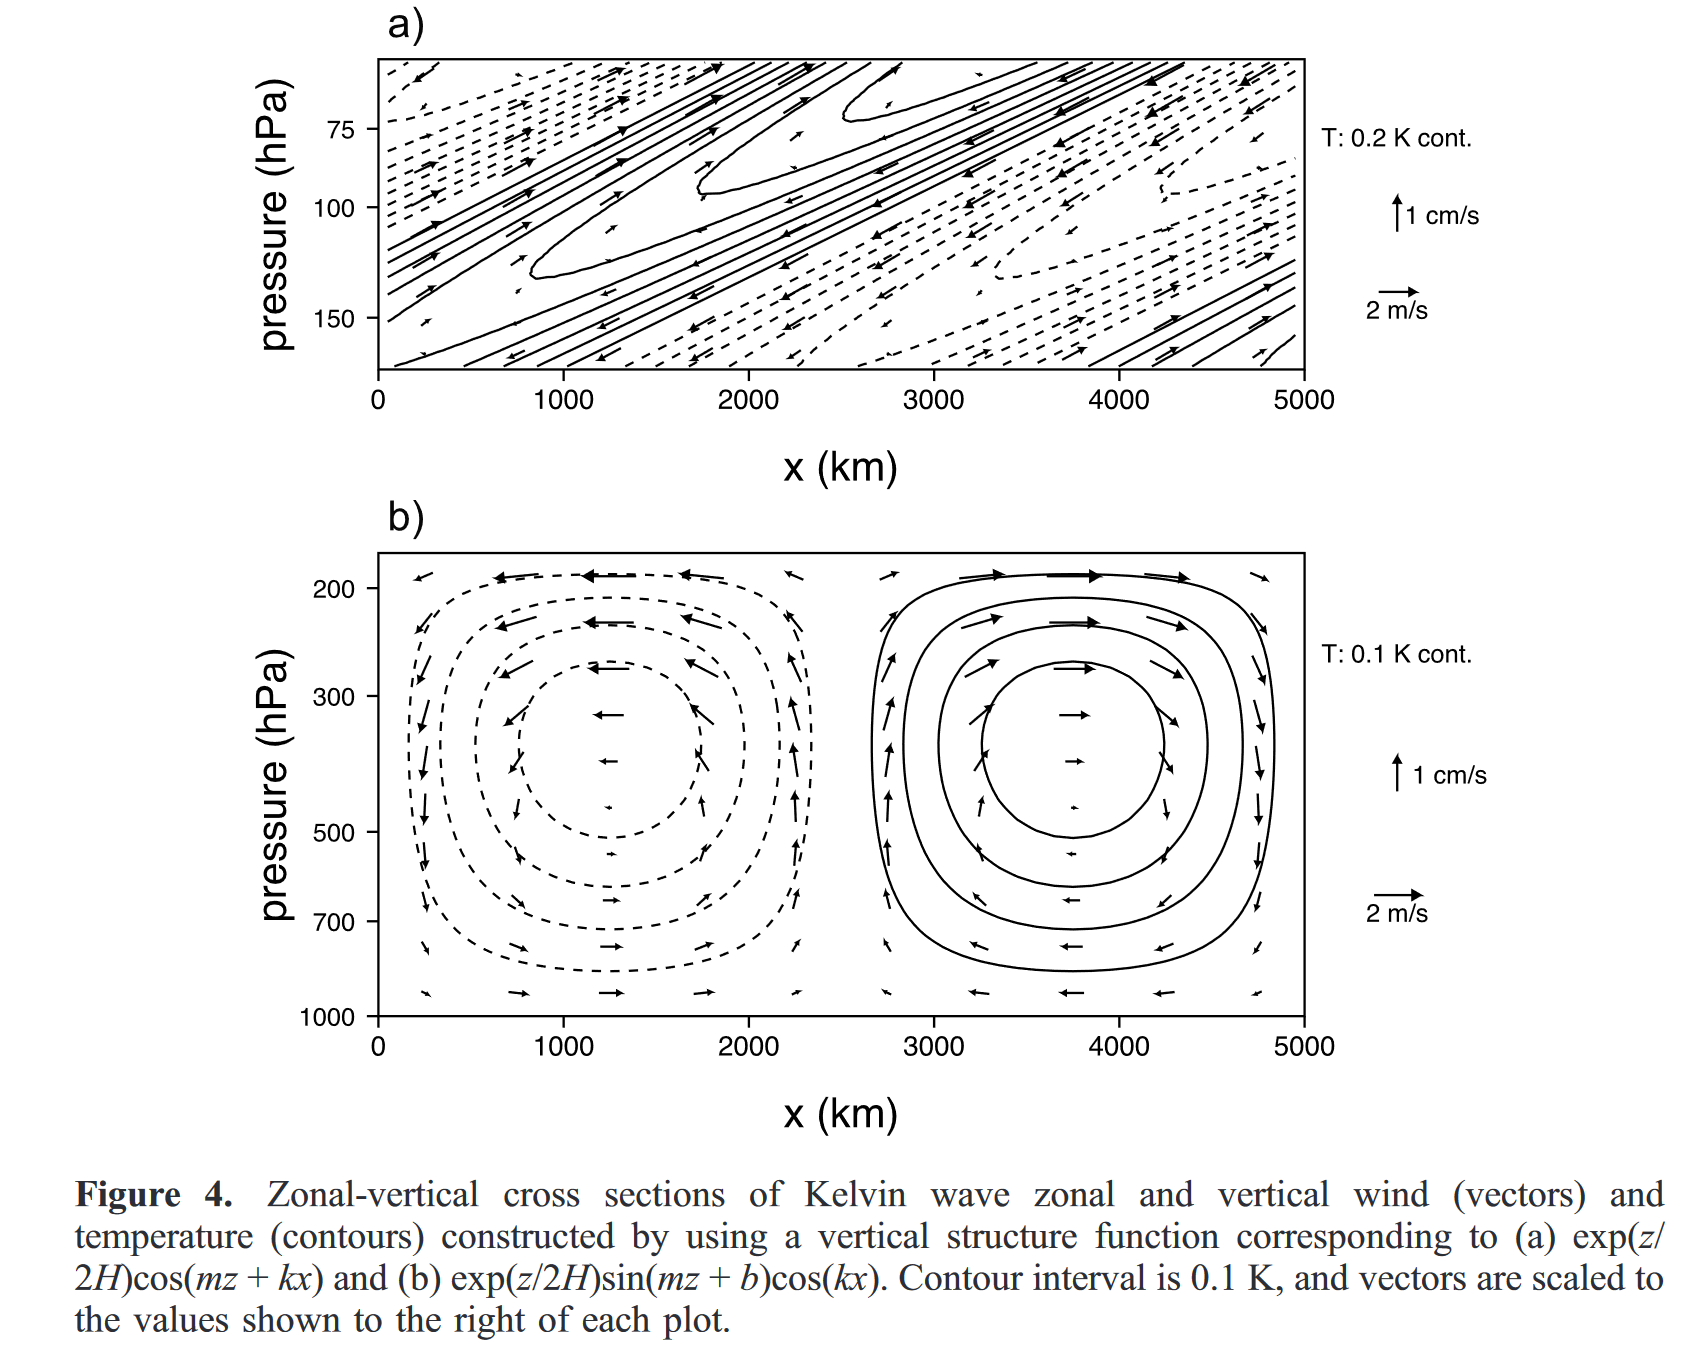
\includegraphics[width=0.75\linewidth]{Fig4.png}

   
\end{figure}


\ 

模式的垂直波长与相应的SW系统的等效深度he之间的关系是这里特别相关的一个话题。在具有恒定稳定度参数N的大气中,垂直模态关于z是正弦的,并对密度随高度的变化进行了修正。例如,通过组合( 12 ),( 14 ),( 15a )和( 15b )得到


\ 

\[m\equiv\frac{2\pi}{L_z}=\left(\frac{N^2}{gh_e}-\frac1{4H^2}\right)^{1/2},\quad\quad\quad(17)\]


\ 

式中:$L_z$为垂直波长。然而,在实际的分层中,模式只是准正弦的,其局部垂直波长在大N (比如在平流层)区域较小,而在低N (例如在对流层[ Fulton and Schubert , 1985 ])区域较大。对于两种不同的代表性分层,表1给出了给定他所对应的局部垂直波长的实例值。


\ 

\paragraph*{2.2.2 湿波}

\ 

有很多方法可以将水分的影响纳入赤道波的理论处理中; 因此,完整的讨论超出了本文的范围。 这里我们简单地解决这个问题:包含凝结加热和冷却是否可以解释观测到的CCEW等效深度与具有类似对流层垂直结构的干波等效深度之间的差异? 对(10)的检查提供了这个问题的答案。 首先,假设该方程中包含非绝热强迫项 $Q$(请记住 $\partial \phi / \partial z$ 与温度扰动成正比):


\ 

\[\frac\partial{\partial t}\left(\frac{\partial\phi}{\partial z}\right)+wN^2=Q.\quad\quad\quad\quad\quad\quad(18)\]


\ 


此外,假设加热扰动与向上运动扰动成正比,即 $Q=\alpha w N^2$(其中 $\alpha$ 是任意常数),这一想法得到了观测支持[Haertel and Kiladis, 2004; Haertel et al., 2008]. 那么(18)就变成了

\ 

\[\frac\partial{\partial t}\left(\frac{\partial\phi}{\partial z}\right)+w(1-\alpha)N^2=0.\quad\quad\quad\quad(19)\]


\ 

在这种情况下,加热有效地降低了气氛的稳定性。 如果 $\alpha$ 接近但略小于 1(即扰动冷凝 加热/冷却消除了由于垂直运动引起的大部分但不是全部温度变化),则大气的“有效静态稳定性”可能会降低到足以 使波动等效深度的理论预测与 CCEW 的观测结果一致 [Gill, 1982b]。 解释 CCEW 等效深度的问题被简化为确定 $\alpha$的理论值,这可以通过使用总湿稳定性概念来完成第一斜压模式(即对流层中具有半垂直波长的模式)[Neelin and Held, 1987; Emanuel et al., 1994; Yu et al., 1998; Haertel and Kiladis, 2004],这本质上是由于\textbf{对流加热和冷却而导致大尺度大气“感觉到”的稳定性降低}。 然而,这种湿波的垂直结构与观测到的CCEW的垂直结构之间仍然存在重要差异。


\ 

\subsection*{ MIXED ROSSBY-GRAVITY WAVES 混合罗斯贝重力波}

\ 

MRG波是Matsuno[1966]预测的赤道波动模态中第一个被观测到,通过对平流层无线电探空数据中的风的波动进行检查[Yanai and Maruyama, 1966; Maruyama, 1967]。后续的研究表明,MRG波也存在与对流层,且与对流耦合在一起[Zangvil, 1975; Zangvil and Yanai, 1981],如理论中描述的向西传播。尽管MRG波于东风波EWs不同,但是他们与n=1的赤道罗斯贝波ER似乎共存于一个连续体中,一些扰动相互转换并发展出混合的结构,特别在西太平洋上空更为显著[Takayabu and Nitta, 1993; Dunkerton and Baldwin, 1995; Yang et al., 2007c]。

\ 

\subsubsection*{ 3.1 观测结构}


\ 

图12展示了基于EOF方法展示了这种转换过程,基于全球南北纬30°以内的2-10天带通滤波的OLR数据。

可以发现,环流位于赤道中心,当波动异常向西移动时,他们转换为离开赤道的环流,然后向西北方向传播到菲律宾地区。这是在太平洋上空常见的起源于赤道波动的扰动的序列[Lau and Lau, 1990; Numaguti, 1995; Chang et al., 1996; Sobel and Bretherton, 1999; Straub and Kiladis, 2003b].。


\ 

相对快速的MRG波在对流层上层以及平流层低层占主导地位。虽然这些上层波动最初可能是由对流强迫产生的,但他们一般以干的模态传播。而与对流紧密耦合的MRG波具有相对较浅的等效深度,\textbf{在对流层低层显示出较大的扰动}[Liebmann and Hendon, 1990; Hendon and Liebmann, 1991; Dunkerton, 1993。 

对流耦合 MRG 波出现在反对称 亮温谱的惯性重力波连续谱的向西传播部分,他们在卫星资料中的信号在西太平洋和中太平洋ITCZ地区最为突出。他们\textbf{在北半球夏季和秋季是最强的,尽管有证据表明这些波全球都发生在所有的海洋辐合带中}[Roundy and Frank, 2004a; WK99; WKW00]。

\ 

在西太平洋上空,MRG 波的对流和动力信号以\textbf{ $15-25 m s^{-1}$的速度向西传播},并且通常显示出向东$5 m s^{-1}$ 的能量频散[Takayabu and Nitta, 1993; Hendon and Liebmann, 1991; Dunkerton and Baldwin, 1995; Sobel et al., 2004; WKW00]。


下图展示了850hpa环流pattern与理论结构十分吻合,涡旋以赤道为中心且关于赤道对称,$T_b$信号反对对称。

波长大约9000km

对流在离开赤道的气流中增强,在向赤道的气流中被抑制;离开赤道后,赤道涡旋和相关的$T_b$信号传播的菲律宾的西北部.

图13c中对应的200 h Pa模态\textbf{在垂直方向上表现为强烈的倾斜},涡度和气压模态与850 h Pa模态接近正交。同时,涡旋在赤道以北略有偏移。虽然这种赤道外的涡旋可以被预期为对远离赤道的加热的响应[e.g., Gill, 1980; Mapes, 1998; Sobel and Horinouchi, 2000],但基本流的不对称也可能是一个因素[e.g., Aiyyer and Molinari, 2003]。

\ 


\begin{figure}
    \centering
    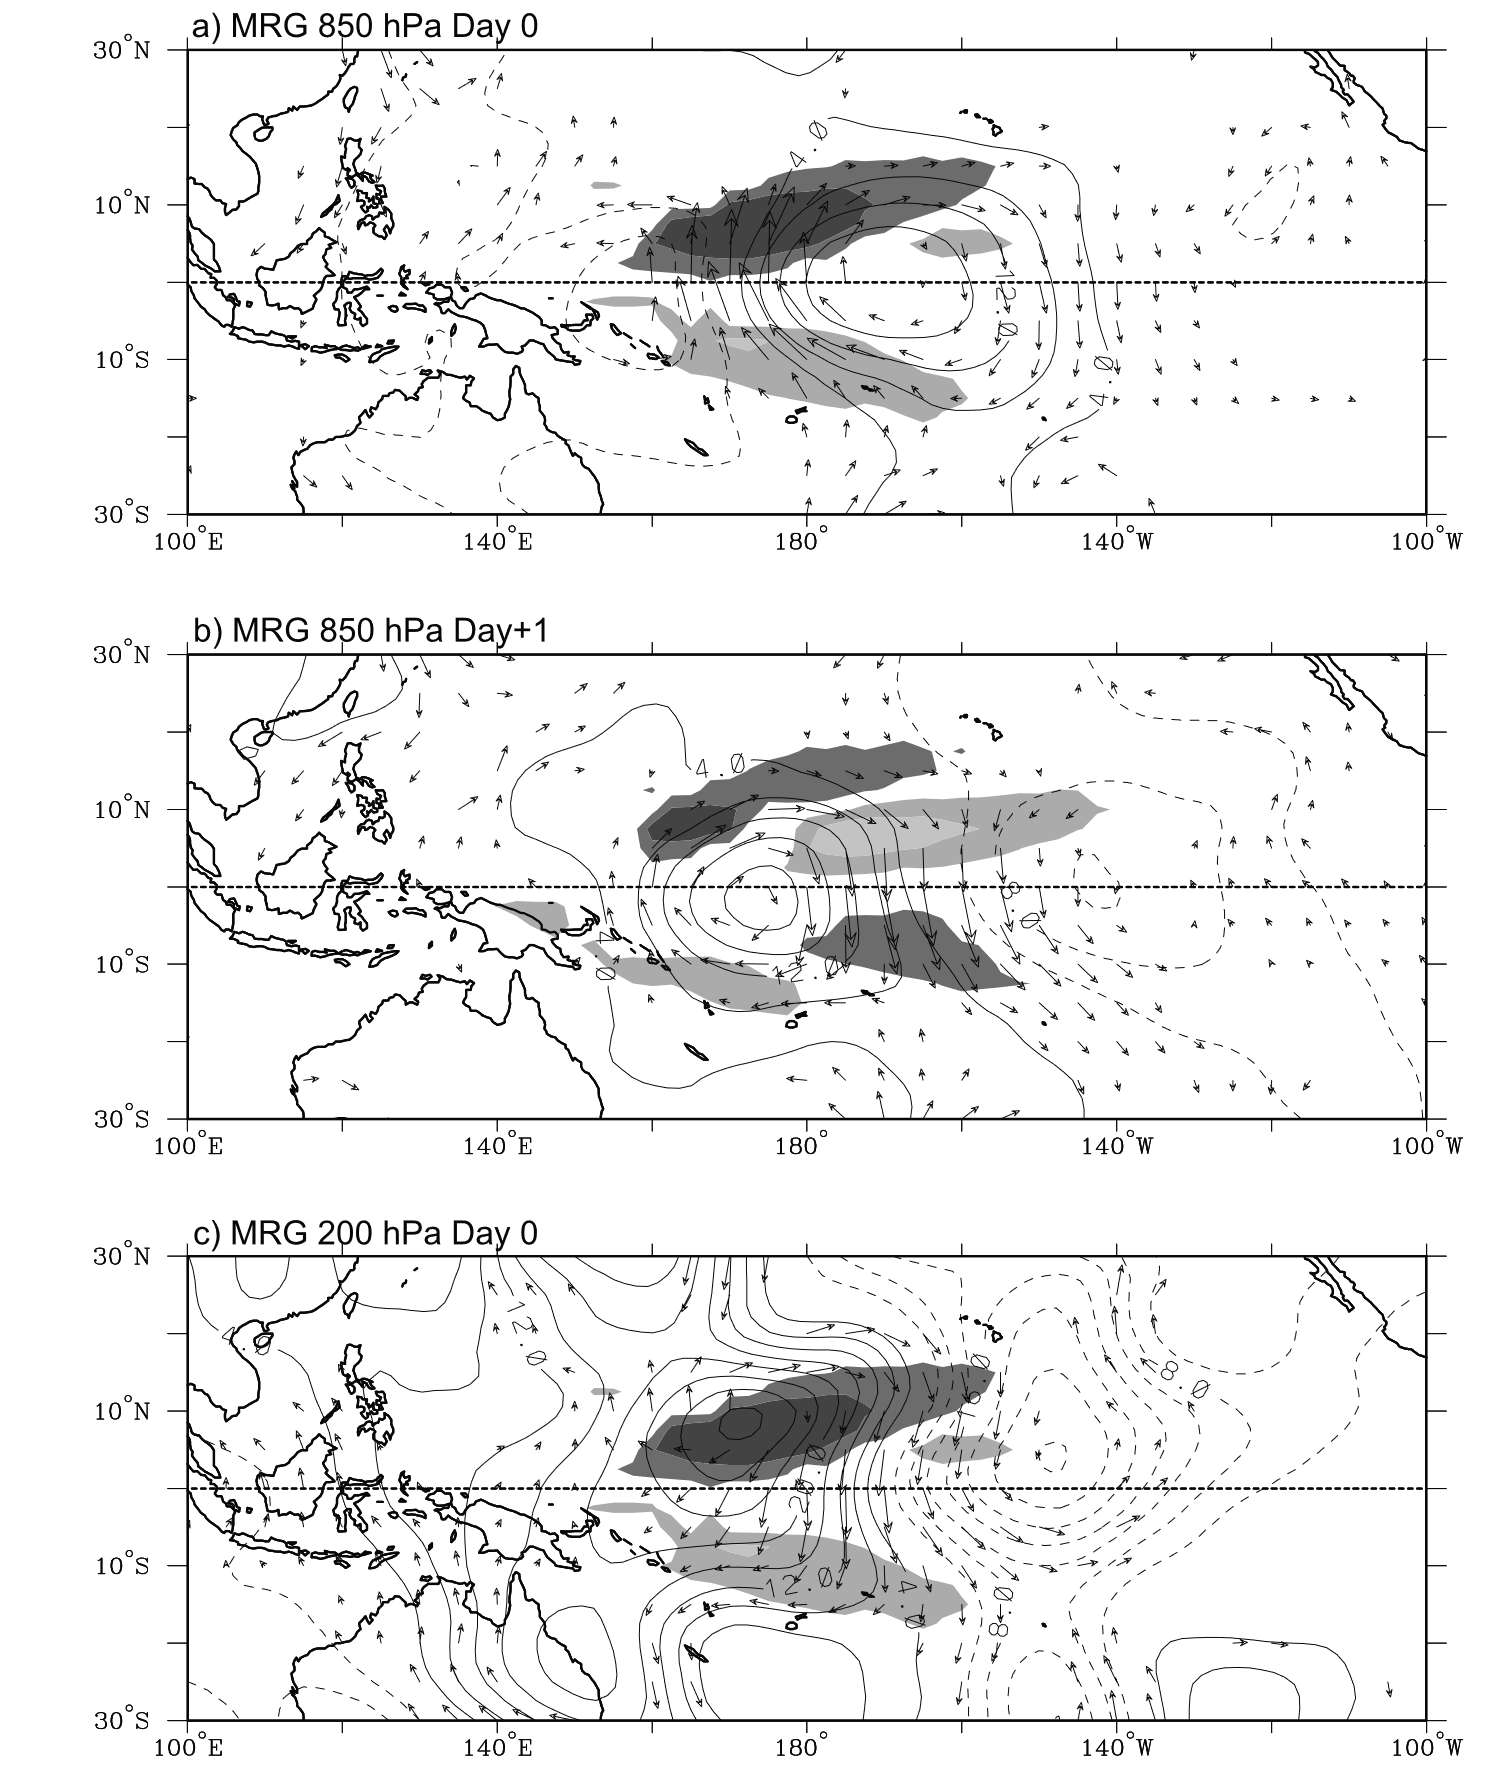
\includegraphics[width=1\linewidth]{Fig13.png}
    \caption{
    Fig13.
    Maps of anomalous Tb (shading), stream function (contours), and wind (vectors) associated with a -20 K perturbation in MRG wave Tb at the base point 7.5°N, 172.5°E, for (a) day 0 at 850 hPa, (b) day +1 at 850 hPa, and (c) day 0 at 200 hPa. The contour interval is $4x10^5 m^2 s^{-1}$, with negative contours dashed. Dark (light) shading is for negative (positive) Tb perturbations of ±10 K and 3 K. Tb and wind vectors are locally significant at the 95% level, with the largest vectors around $4 m s^{-1}$.}
   }
\end{figure}



\ 
MRG波经向风的垂直倾斜结构已经被证实,如图14所示。$T_b$最低时刻的对流层低层向极流从地面至750 h Pa左右,然后向东倾斜至200 h Pa左右,对流层高层和平流层低层则相反。





\ 
\begin{figure}
    \centering
    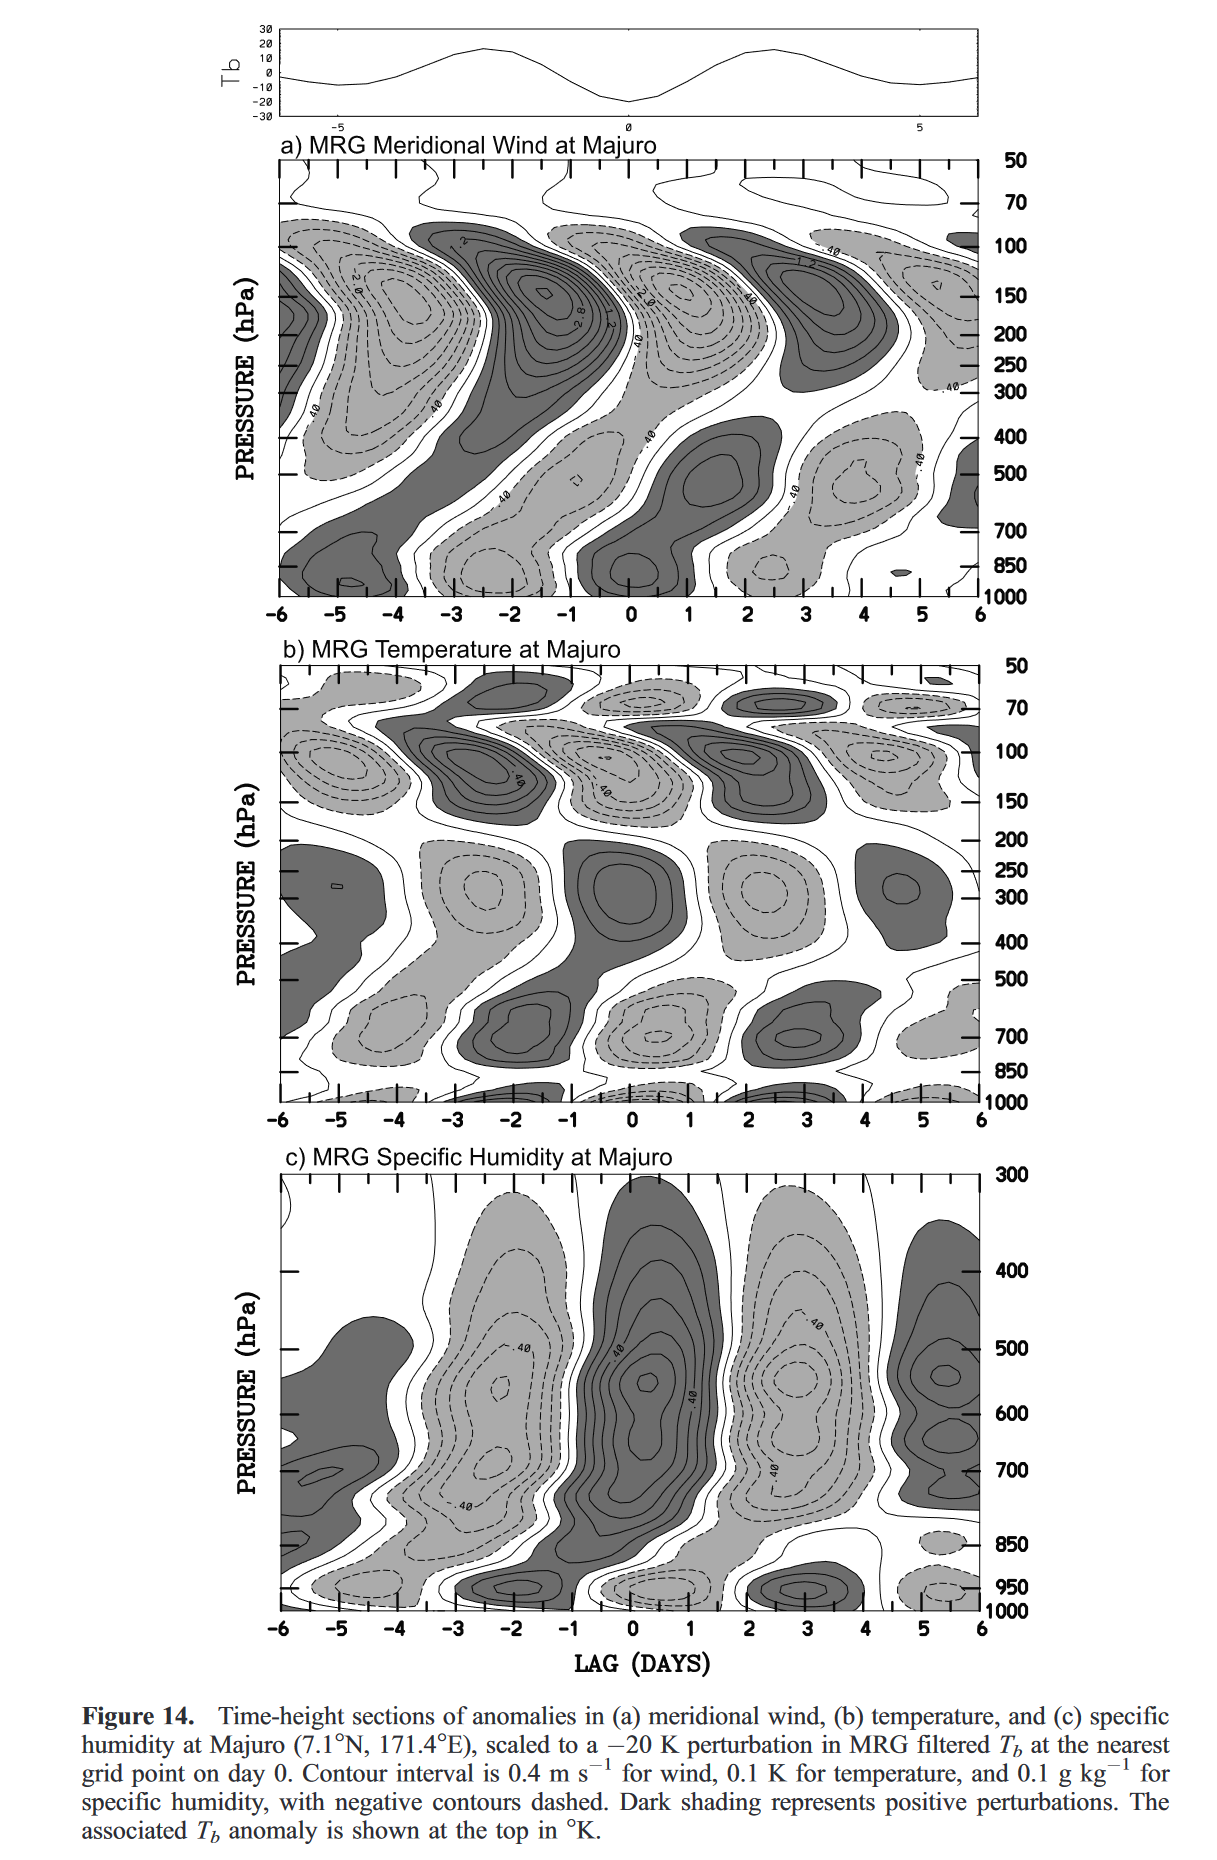
\includegraphics[width=1\linewidth]{Fig14.png}

\end{figure}

\subsubsection*{3.2 MRG波的影响}

当逆时针旋转的MRG波涡旋,当他们移出赤道并成为以气旋性涡旋为中心时,有利于进一步发展为热带气旋Frank and Roundy [2006]。在个别气旋的形成过程中,观察到了这样的序列Dickinson and Molinari [2002], Straub and Kiladis [2003b], and Zhou and Wang [2007]。

这种MRG波向小尺度结构的转变,被认为受到了纬向流交汇区的正压变形的帮助,\textbf{低层西风和东风在西太平洋上空交汇,导致纬向收缩和更小尺度的赤道外罗斯贝涡旋的发展}[Kuo et al., 2001; Aiyyer and Molinari, 2003]。

\begin{tcolorbox}[colback=yellow!20, boxrule=0pt, sharp corners]
\textcolor{yellow!70!black}{这种辐合也可能是扰动通过“波能累积”的机制导致放大[e.g., Farrell and Watterson, 1985; Webster and Chang, 1988].其中波的纬向群速度趋近于零,从而俘获了波的能量,创造了有利于热带气旋形成的环境[Holland, 1995; Sobel and Bretherton, 1999]}
\end{tcolorbox}


在印度扇区[Bessafi and Wheeler, 2006]上空也有一些与MRG相关的热带气旋生成的证据,如图5所示。通过温带Rossby波在MRG结构上的投影,横向强迫激发MRG波,正如第4节讨论的Kelvin波一样,也被观测到的[Magan ̃a and Yanai, 1995]和理论上的[Hoskins and Yang, 2000]所支持。

\ 


\subsection*{EWs 东风波}


\ 虽然不是Matsuno[1966]的赤道浅水方程中的解,但是是第一个被证实的对流耦合波动。表现为:赤道外向西传播的罗斯贝涡旋在北半球赤道辐合带的信风场内表现为气压和风的"倒槽" 。
主要活跃在太平洋和大西洋,以及季风季节的撒哈拉沙漠以南的非洲。在ITCZ对流最活跃的季节时空谱中,东风波的信号最显著(5-10 月 )(WK99).。


早期观测研究发现,EWs的波长为2500-3500km,西传相速度为$8m s^{-1}$
,周期为3-4天,最大经向风速异常在700-850hPa[Reed and Recker, 1971; Reed et al., 1977; Thompson et al., 1979]。在西非/东大西洋地区,对流的位相和波动特性随着纬度以及陆地和海洋之间的变化而变化[Reed et al., 1977; Kiladis et al., 2006]。此外, 也有研究表明太平洋EWs的特征随着经度的变化而变化[Reed and Recker, 1971; Tam and Li, 2006; Serra et al., 2008]。


大部分的观测中发现的太平洋EWs结构变化归因于\textbf{整个太平洋背景平均垂向风切变的变化}引起的[Holton, 1971; Reed and Recker, 1971]。水平和垂向风切变也强烈影响了非洲EWs的结构,同时其与热带气旋之间的关系被归因于纬向变化的纬向气流中的形变和波能积累的作用。
\ 相反,热带气旋产生的Rossby波能量的向东频散被证明是EWs的一个来源[Holland, 1995; Sobel and Bretherton, 1999; Krouse et al., 2008],以及热带外强迫[Tam and Li, 2006]和非洲东风急流区域内的潜热加热[e.g., Hsieh and Cook, 2007; Thorncroft et al., 2008]的潜在影响。

EWs的垂向结构和尺度与MRG波十分相似,几乎难以区分[see Kiladis et al., 2006; Serra et al., 2008]。对非洲上空EWs的能量分析表明强的斜压转换使得从非洲东风急流内部的垂直切变中获取能量[Norquist et al., 1977; Kiladis et al., 2006; Hall et al., 2006; Hsieh and Cook, 2007]。随着EWs离开海岸,正压转换变得更占优势,能量主要从基本态水平剪切中提取。在太平洋ITCZ,基本态的水平和垂直切变要少得多,能量学计算表明\textbf{潜热加热一定是太平洋EWs的主要能量来源} [Tai and Ogura, 1987; Lau and Lau, 1992; Tam and Li, 2006; Serra et al., 2008]。
虽然\textbf{潜热加热可能是大多数CCEW的主要能量来源,但强切变的存在,特别是在季风区,可能对它们的产生和维持也很重要 }。




参考:
Kiladis, G. N., M. C. Wheeler, P. T. Haertel, K. H. Straub, and P. E. Roundy (2009), Convectively coupled equatorial waves, Rev. Geophys., 47, RG2003, doi:10.1029/2008RG000266 



\ 






\ 






\ 





\ 

\begin{figure}
    \centering
    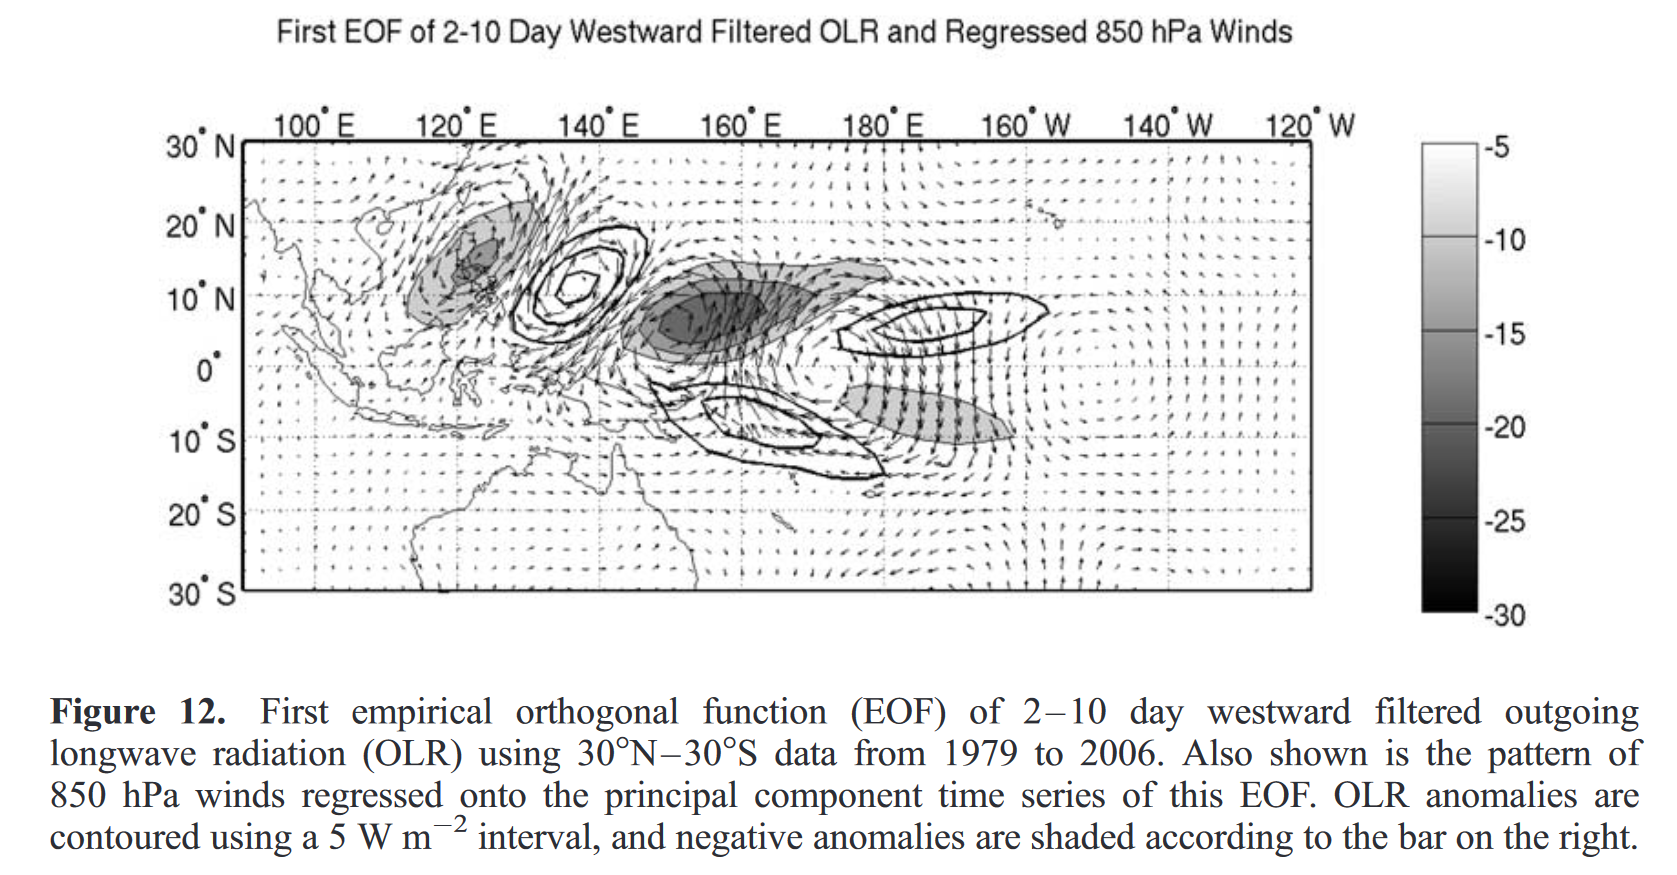
\includegraphics[width=1\linewidth]{Fig12.png}

\end{figure}


\ 




\ 




\ 




\ 




\ 




\ 




\ 




\ 




\ 




\ 




\ 




\ 




\ 




\ 




\ 




\ 




\ 




\ 




\ 




\ 




\ 




\ 




\ 




\ 




\ 




\ 




\ 




\ 




\ 




\ 




\ 




\ 




\ 




\ 




\ 




\ 




\ 




\ 




\ 




\ 




\ 




\ 




\ 




\ 




\ 




\ 




\ 




\ 



\ 




\end{CJK*}
\end{document}

